\section{Прикладная задача поиска оптимального управления}
\label{sec:optimal_cpntrol}
Задача глобальной оптимизации возникает при синтезе оптимальных с точки зрения некоторых
критериев управлений в линейных системах ОДУ. Если управление является линейной обратной
связью по состоянию, то система с управлением имеет вид:
\begin{equation}
  \label{eq:control_system}
    \dot x = (A+B_u\Theta)x + B_v v, x(0)=0,
\end{equation}
где  \(v(t)\in L_2\) --- некоторое возмущение.
Выходы системы описываются формулами \(z_k=(C_k+B_u\Theta),k=\overline{1,N}\).
Вляиние возмущения на \(k\)-й выход системы описывается критерием
\begin{displaymath}
  J_k(\Theta)=\sup_{v\in L_2} \frac{\max_{1\le i \le n_k} \sup_{t\ge 0}|z_k^{(i)}(\Theta,t)|}{||v||_2}.
\end{displaymath}

Нужно найти компоненты вектора \(\Theta\), минимизирующие один из критериев при
заданных ограничениях на другие:
\begin{displaymath}
   J_1(\Theta^*)=\min\{J_1(\Theta):J_k(\Theta)\leqslant S_k,k=\overline{2,N}\}.
\end{displaymath}

В \cite{optControl} указан способ вычисления критериев, состоящий в следующем:
\begin{itemize}
\item найти матрицу \(Y\) из уравнения:
\begin{displaymath}
  (A+B_u\Theta)Y+Y(A+B_u\Theta)^\mathsf{T}+B_v B_v^\mathsf{T} = 0
\end{displaymath}
\item если \(Y\) положительно определена, то используя её, вычислить функционалы \(J_k(\Theta)\):
\begin{displaymath}
  J_k(\Theta)=\sqrt{\max_{1\leqslant i\leqslant n_k}\{(C_k^{(i)}+D_k^{(i)}\Theta)Y(C_k^{(i)}+D_k^{(i)}\Theta)^\mathsf{T}\}},k=\overline{1,N},
\end{displaymath}
где \(C_k^{(i)},D_k^{(i)}\) --- \(i\)-е строки матриц \(C_k\) и \(D_k\) соответственно.
\end{itemize}

Для предотвращения случаев, когда \(Y\) незнакоопределена, в качестве дополнительного ограничения
использовался критеий устойчивости линейной системы ОДУ: все действительные части
собственных чисел матрицы \(A+B_u\Theta\) должны быть отрицательны:
\begin{displaymath}
  g_0(\Theta)=\min_{j}\re(\lambda_j(\Theta)) < 0
\end{displaymath}

С целью проверки корректности реализации вычисления критериев задачи
индексным алгоритмом глобального поиска были решены две задачи рассматриваемого типа
(их решение также приведено и в \cite{optControl}).

В задаче виброзащиты параметры системы (\ref{eq:control_system}) определются следующим
образом:
$$
A=\begin{bmatrix}
    0       & 1 \\
    0       & 0 \\
\end{bmatrix},
B_v=B_u=\begin{bmatrix}
  0       \\
  1       \\
\end{bmatrix},
C_1=\begin{bmatrix}
  0     & 1
\end{bmatrix},D_1=0,
C_2=\begin{bmatrix}
  0     & 1
\end{bmatrix},D_2=1.
$$

Управление имеет вид \(u=[\theta_1,\theta_2]x\), где \(\theta_1 \leqslant 0,\theta_2\leqslant 0\) ---
оптимизируемые параметры. Сама задача ставится следующим образом:
\begin{equation}
  \label{eq:opt_ctrl_problem}
  J_2(\Theta^*)=\min\{J_2(\Theta):J_1(\Theta)\leqslant 1, g_0(\Theta)\leqslant -0.02\}.
\end{equation}

\begin{figure}[ht]
  \center
  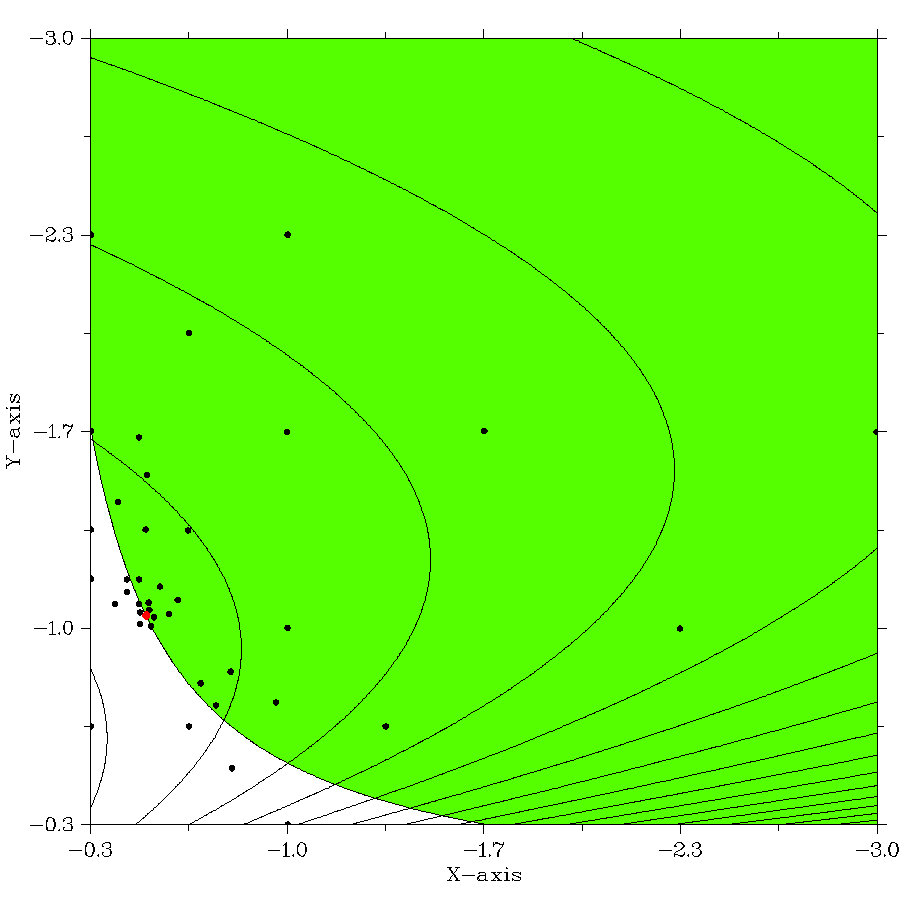
\includegraphics[width=0.55\textwidth]{images/controlProblem.png}
  \caption{Линии уровня для задачи виброзащиты с отмеченными точками испытаний АГП}
  \label{fig:controlProblem}
\end{figure}
При решении этой задачи АГП с параметрами \(r=2.3\), \(\varepsilon=10^{-2}\) произвёл
65 испытаний, причём целевая функция была вычислена 27 раз. Найдена оптимальная точка с координатами
\(\widetilde\theta_1 =-0.503223,\widetilde\theta_2=-0.997168\), \(J_2(\widetilde\Theta)=0.866551\),
а ограничение на \(J_1\) активно.
На рис. \ref{fig:controlProblem}
представлены линии уровня целевой функции задачи виброзащиты. В данном случае допустимая область (закрашена на рисунке)
имеет довольно простую границу, а целевая функция унимодальна.

В задаче гашения колебаний параметры системы (\ref{eq:control_system}) определются следующим
образом:
$$
A=\begin{bmatrix}
  0  & 0 & 1 & 0 \\
  0  & 0 & 0 & 1 \\
  -2  & 1 & -2\beta & \beta \\
  1  & -1 & \beta & -\beta \\
\end{bmatrix}, \beta = 0.1,
B_v=\begin{bmatrix}
0       \\
0       \\
1       \\
1       \\
\end{bmatrix},
B_u=\begin{bmatrix}
0       \\
0       \\
0       \\
1       \\
\end{bmatrix},
$$
$$
C_1=\begin{bmatrix}
1 & 0 & 0 & 0 \\
-1 & 1 & 0 & 0
\end{bmatrix},
D_1=\begin{bmatrix}
0 \\
0
\end{bmatrix},
C_2=\begin{bmatrix}
0 & 0 & 0  & 1
\end{bmatrix},D_2=1.
$$

Управление имеет вид \(u=[\theta_1,\theta_2, \theta_3,\theta_4]x\), где \(\theta_1,\theta_2, \theta_3,\theta_4\) ---
оптимизируемые параметры. Сама задача ставится так же, как и предыдущая:
\begin{displaymath}
  J_2(\Theta^*)=\min\{J_2(\Theta):J_1(\Theta)\leqslant 1, g_0(\Theta)\leqslant -0.02\}.
\end{displaymath}

В процессе решения этой задачи АГП c указанными ранее параметрами сделал 336575 испытания, причём целевая функция
была вычислена 5173 раза. Найдена оптимальная точка с координатами
\(\widetilde\theta_1 =0.322954,\widetilde\theta_2=-0.583130, \widetilde\theta_3=-0.453491, \widetilde\theta_4=-0.970581\),
\(J_2(\widetilde\Theta)=1.056579\), а ограничение на \(J_1\) активно.

Рассмариваемые задачи поиска оптимального управления по состоянию интересны, пержде
всего, в многокритериальной постановке. В данной работе рассматриваются
задачи с двумя критерими: один отвечает за максимальное смещение колебательного объекта,
а другой --- за максимальное управляющее воздействие. Для отыскания Парето-границы на
плоскости критериев достаточно воспользоваться постановкой (\ref{eq:opt_ctrl_problem}).
Варьируя максимальное значение критерия \(J_1(\theta)\) и каждый раз убеждаясь, что
ограничение на \(J_1(\theta)\) активно, мы получим пары \((J_1,J_2)\), соответствующие
Парето-границе. Этот метод неприменим в случае, когда одному значению \(J_1\)
соответствует несколько значений \(J_2\), лежащих на Парето-границе (то есть в
границу входит вертикально ориентированный отрезок). При применении этого метода в задаче,
которая будет описана далее, не было выявлено каких-либо непердвиденных разрывов и резких скачков кривой-границы,
поэтому другие способы решения многокритериальных задач не рассматривались.

Задача, в которой требовалось найти Парето-границу является расширением упомянутой ранее
задачи виброзащиты, однако объект защиты представлен многомассовой механической системой.
Приведём уравнения, описывающую двухмасовую систему:
\begin{displaymath}
  \begin{array}{cr}
    \begin{cases}
      \dot x_1 = x_3 \\
      \dot x_2 = x_4 \\
      \dot x_3 = -x_1 + x_2 - \beta x_3 + \beta x_4 + u + v \\
      \dot x_4 = x_1 - x_2 + \beta x_3 - \beta x_4 + u
    \end{cases} \\
    x_1(0)=x_2(0)=x_3(0)=x_4(0)=0
\end{array}
\end{displaymath}

В случае \(n\)-массовой системы матирцы из (\ref{eq:control_system}) определяются
следующим образом:
$$
A=\begin{bmatrix}
  0_{n \times n}  & I_n\\
  -K  & -\beta K\\
\end{bmatrix}, \beta = 0.1,
B_v=\begin{bmatrix}
0_{n\times 1}       \\
p       \\
\end{bmatrix},
B_u=\begin{bmatrix}
0_{n\times 1}       \\
q       \\
\end{bmatrix},
p = \begin{bmatrix}
1 \\
1 \\
\dots \\
1 \\
\end{bmatrix},
q = \begin{bmatrix}
1 \\
0 \\
\dots \\
0 \\
\end{bmatrix},
$$
$$
K = \begin{bmatrix}
  1  & -1 & 0 & \dots & \dots & 0\\
  -1  & 2 & -1 & \dots & \dots & 0\\
  \dots  & \dots & \dots & \dots & \dots & \dots\\
  \dots  & \dots & \dots & -1 & 2 & -1\\
  \dots  & \dots & \dots & 0 & -1 & 1\\
\end{bmatrix},
$$
$$
C_1=\begin{bmatrix}
1 & 0 & \dots & 0 & 0 & 0 \\
\end{bmatrix},
D_1=\begin{bmatrix}
0 \\
\end{bmatrix},
C_1=\begin{bmatrix}
-1 & 1 & 0 & \dots & 0 & 0 \\
0 & -1 & 1 & \dots & 0 & 0 \\
\dots & \dots & \dots & \dots & \dots & \dots \\
0 & \dots & \dots & \dots & 0 & 0 \\
0 & \dots & -1 & 1 & \dots & 0 \\
\end{bmatrix},
D_2=\begin{bmatrix}
0 \\
0 \\
\dots \\
0 \\
0
\end{bmatrix},
$$
где \(K\in \mathbf{R}^{n\times n};\; p,q\in \mathbf{R}^{n}\), \(C_1\in \mathbf{R}^{1\times 2n}, C_2\in \mathbf{R}^{n-1\times 2n}\),
\(D_2 \in \mathbf{R}^{1\times 2n}\).

Будем рассмаривать описанную задачу при \(n=10\). В отличие от ранее приведённых задач в управление
включены не все фазовые переменные, а только три из них: \(u=\theta_1 x_1 + \theta_2 x_3 + \theta_3(x_2-x_3), \theta_1 \leqslant 0, \theta_2\leqslant 0\).
Таким образом, решаемая задача оптимизации является трёхмерной. Если считать систему
полностью наблюдаемой, то количество переменных увеличится до 20.

В \cite{optControl} показано, что при полностью наблюдаемом состоянии системы Парето-граница
в рассматриваемой задаче может быть получена с использованием линейных матричных
неравенств. Кривая \(\gamma_{inf}\), полученная коллегами с кафедры Кафедра Дифференциальных уравнений, математического и численного анализа,
представлена на рис. \ref{fig:pareto}. При её построении на абсолютные значения компонент
вектора \(\Theta\) не накладывалось никаких ограничений, поэтому её можно считать
некоторой предельной, идеальной кривой, которая нереализуема в реальной системе.

\begin{figure}[ht]
    \center
    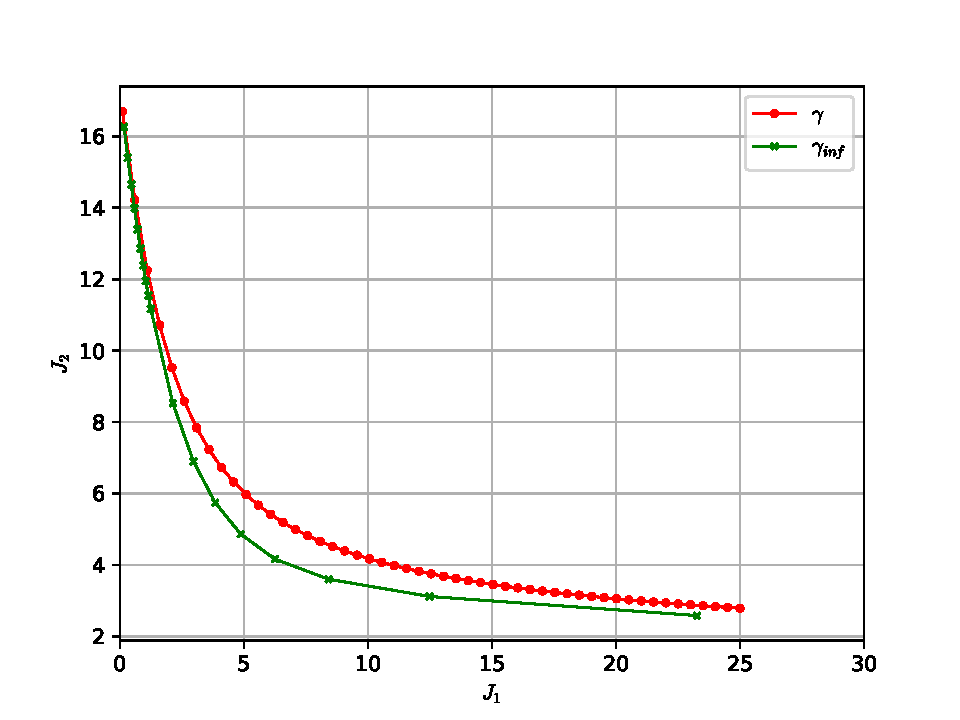
\includegraphics[width=0.75\textwidth]{images/solution.pdf}
    \caption{Парето-границы в задаче виброизоляции при \(n=10\), построенные для
    частично и полностью наблюдаемого состояния}
    \label{fig:pareto}
\end{figure}

Построенная c помощью системы Globalizer описанным ранее способом Парето-граница
показана на рис. \ref{fig:pareto} (кривая \(\gamma\)). При её построении были ограничены
абсолютные значения коэффициентов обратной связи: \(|\theta_i|<10^4\). Сравнивая
кривые \(\gamma_{inf}\) и \(\gamma\), можно сказать, что потеря качества управления при неполной наблюдаемости
и ограниченных коэффициентов обратной связи некритическая.
